\chapter{Conclusions}
\label{chp-conclusions}

In this report, we explore the development of finite volume methods from one dimension to two dimensions,
examining their application on both the plane and the cubed-sphere.
We elucidate that on the cubed-sphere, the finite volume approach for solving the advection equation simplifies to solving the two-dimensional
advection equation independently on each panel, akin to the plane.
However, it incorporates the inclusion of the metric tensor and boundary conditions that depend on the adjacent panels.
The key disparity between methods on the plane and the sphere lies in the formulation of the metric tensor term and the computation of stencils at ghost cell positions.


In Chapter \ref{chp-1d-fv}, we present an overview of 1D finite volume schemes with slope limiters (FV-SL) for the advection equation.
We discuss three essential tasks: function reconstruction, determination of control volume edges' departure points, and flux computation.
For accurate reconstruction, we employed the PPM method and its variations to ensure monotonicity.
Departure point calculation methods include RK1 and a two-stage Runge-Kutta scheme (RK2).
Flux computation involves integrating the reconstructed function over a domain determined by the departure point.
Numerical experiments demonstrate that a PPM variant, namely PPM-PL07 from \citet{putman:2007}, which utilizes fifth-order reconstruction,
outperforms the original PPM \citep{colella:1984}. Monotonic schemes, such as PPM-L04 and PPM-CW84, prevent overshoots, with PPM-L04 being more accurate.
When subjected to variable velocity tests, the RK1 scheme exhibits a first-order error despite its third-order accuracy in space,
while the RK2 scheme maintains third-order accuracy. Combining PPM-PL07 with RK2 ensures at least second-order accuracy.

In Chapter \ref{chp-2d-fv}, we introduce the dimension-splitting method as a cost-effective approach for solving the 2D advection equation.
This method replaces the 2D problem with multiple 1D advection equations using a 1D finite volume scheme with slope limiters based on PPM.
We modified the average of two Lie-Trotter splittings (AVLT) to ensure the preservation of a constant scalar field with a divergence-free velocity,
resulting in the PL07 splitting proposed by \citet{putman:2007} and the L04 splitting proposed by \citet{lin:2004}.
Our conclusion from this chapter is that the PL07 splitting combined with the RK1 schemes yields the most accurate results but only first order,
while the AVLT splitting achieves second-order when employed with the RK2 scheme.

In Chapter \ref{chp-cs-grids}, we explored cubed-sphere mappings, particularly the equiangular mapping, which generates a more uniform grid.
A key feature of equiangular cubed-sphere ghost cells is that their edge and center ghost points align with a common geodesic, alongside adjacent panel points.
This property enables us to employ 1D Lagrange interpolation for obtaining field values in the ghost cells, as demonstrated through numerical examples.
We compared this ghost cell treatment, referred to as ET-ZA22, with an extrapolation method called ET-PL07 proposed by \citet{putman:2007},
as well as a scheme that disregards panel discontinuities.
We observed that among these methods, only ET-ZA22, utilizing edge reconstruction from PPM, avoided the creation of grid-imprinting patterns.
The PL07 scheme exhibited second-order accuracy but generated significant grid imprinting patterns.

In Chapter \ref{chp-cs-fv}, we extended the dimension splitting technique from Chapter \ref{chp-2d-fv} 
to each cubed-sphere panel by incorporating the edge treatment schemes discussed in Chapter \ref{chp-cs-grids}.
We highlighted that the ET-ZA22 scheme breaks mass conservation and proposed two approaches to address this issue:
one involving averaging the flux at the cube edges (ET-ZA22-AF), and the other involving projecting the divergence
onto the space of grid functions with zero mass (ET-ZA22-PR).
Numerical experiments revealed that ET-ZA22-AF reduced the order near the edges and produced a grid imprinting pattern,
whereas ET-ZA22-PR preserved the scheme order and eliminated any grid imprinting pattern.
Additionally, we investigated two formulations of the metric tensor in the flux, one with its incorporation in the PPM reconstruction (MT-0) and the other without it (MT-PL07).
For experiments without the metric tensor, we employed the PL07 splitting with RK1 and utilized the edge treatments ET-ZA22-PR and ET-PL07.
It became evident that ET-ZA22-PR improved the accuracy of the method and reduced grid imprinting. However, in the steady test case, we notice that the ET-ZA22-PR may still
generate a small grid-imprinting.

\newpage
\section{Future work}
The next steps of this work can be divided into two main aspects.
Firstly, we propose to expand upon the analysis presented in Chapter \ref{chp-cs-fv},
where our objective is to implement the FV3 shallow-water core on the cubed-sphere based on the approach described by \citet{lin:1997}.
The computational implementation of this step is expected to be relatively straightforward,
as the shallow-water model already includes flux operators that have been implemented using
standard finite-difference operators. Our goal is to assess the accuracy of this scheme,
investigate grid imprinting at the edges, and explore potential methods for enhancing the performance of the scheme.

\begin{figure}[!htb]
	\centering
	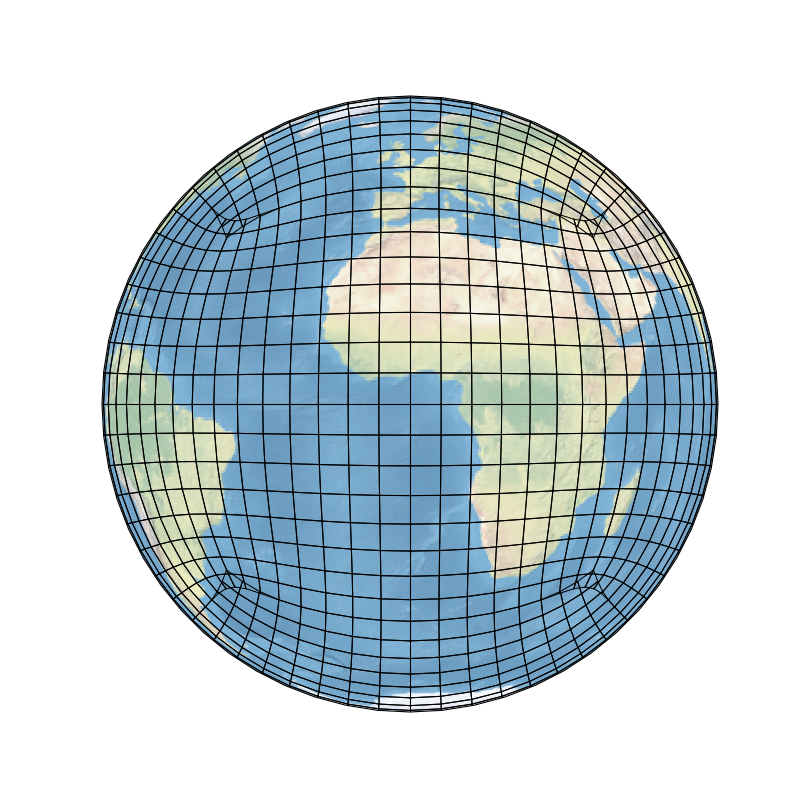
\includegraphics[width=0.4\linewidth]{overlapped_cs_16_sphere.png}
	\caption{Overlapping cubed-sphere.\label{gridoverlaped}}
\end{figure}

In our second proposal, we aim to extend the FV3 shallow-water core to the overlapping cubed-sphere grid, a grid proposed by \citet{purser:2017}, shown in Figure \ref{gridoverlaped}.
This grid offers several advantages, including an orthogonal coordinate system and an abundance of cells at the cubed-edge,
which enables the utilization of neighboring panel information without interpolation or extrapolation, potentially reducing grid imprinting.
Also, the overlapping region is very small.
The main challenge lies in effectively dealing with the overlapped region of the grid. To tackle this issue, we plan to explore methods used in the Yin-Yang grids, which also have overlapping regions and are currently implemented in the Global Environmental Multiscale (GEM) model by Canada \citep{qaddouri:2011,husain:2019}.
Additionally, we intend to investigate existing methods developed for overlapping grids, which have been widely employed in the finite-volume literature for representing complex geometries
(see for instance \citet{hadzic:2005}).
This research will contribute to enhancing our understanding of overlapping grids and aid in the development of effective techniques for the overlapping cubed-sphere grid.

